\begin{frame}{BLIP: One Model for Understanding and Generation}
  \begin{columns}[T,onlytextwidth]
    \column{0.55\textwidth}
      \begin{itemize}\footnotesize\itemsep0.35em
        \item \textbf{BLIP} (Li et al., ICML 2022) addresses two weaknesses of vision-language pretraining at the time.
        \item \textbf{Model:} encoder-based models (CLIP, covered earlier; ALBEF) are hard to transfer directly to captioning; encoder-decoder models had not been adopted successfully for retrieval.
        \item \textbf{Data:} gains came largely from scaling up web alt-texts, which ``often do not accurately describe the visual content of the images'' (Sec.~3.3).
        \item \textbf{ALBEF} (Li et al., NeurIPS 2021), the predecessor: contrastive alignment of image and text features before cross-attention fusion, plus soft targets from a moving-average copy of the model.
        \item \textbf{BLIP's answers:} the multimodal mixture of encoder-decoder (\textbf{MED}) and captioning and filtering (\textbf{CapFilt}).
      \end{itemize}
    \column{0.43\textwidth}
      \centering
      \vspace{1.2em}
      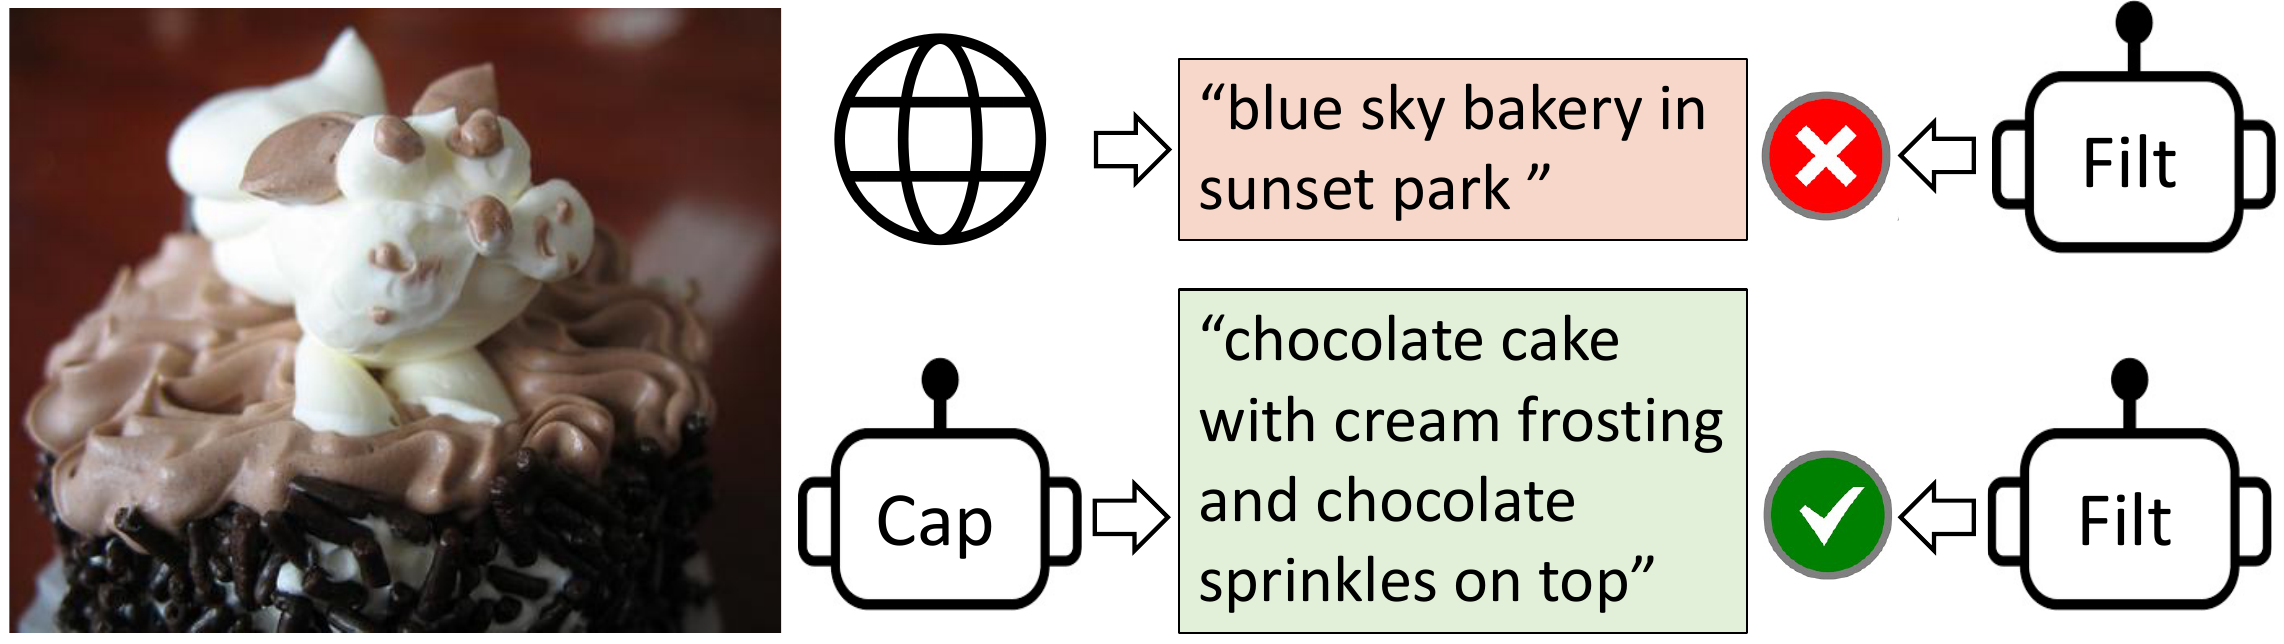
\includegraphics[width=\linewidth,height=0.40\textheight,keepaspectratio]{images/vision-language-models/blip_fig1_capfilt_example.png}\\[0.3em]
      {\scriptsize ``We use a Captioner (Cap) to generate synthetic captions for web images, and a Filter (Filt) to remove noisy captions.'' Li et al., ``BLIP: Bootstrapping Language-Image Pre-training for Unified Vision-Language Understanding and Generation,'' ICML 2022, \href{https://arxiv.org/abs/2201.12086v2}{arXiv:2201.12086v2}, Figure~1.\par}
  \end{columns}
\end{frame}

\begin{frame}{Multimodal Mixture of Encoder-Decoder}
  % images/vision+text/captioning-blip.png is Figure 2 of arXiv:2201.12086v2.
  \centering
  \includegraphics[width=\linewidth,height=0.45\textheight,keepaspectratio]{images/vision+text/captioning-blip.png}\\[0.1em]
  {\scriptsize ITC: image-text contrastive loss; ITM: image-text matching; LM: language modeling; ``same parameters have the same color''. Li et al., \href{https://arxiv.org/abs/2201.12086v2}{arXiv:2201.12086v2}, Figure~2.\par}
  \vspace{0.3em}
  \begin{itemize}\footnotesize\itemsep0.15em
    \item ViT-B/16 or ViT-L/16 image encoder; the text Transformer starts from BERT-base, a Transformer text encoder pretrained by predicting masked words. A task-specific first token, [CLS], [Encode] or [Decode], marks the mode.
    \item The grounded encoder adds a cross-attention layer (covered earlier) between self-attention and feed-forward in every block; the decoder makes self-attention causal.
    \item \textbf{Sharing} all text layers except self-attention: 252M parameters against 361M unshared, at equal or better scores; sharing self-attention too lowers every score (Table~3).
  \end{itemize}
\end{frame}

\begin{frame}{Three Objectives per Image-Text Pair}
  \begin{itemize}\footnotesize\itemsep0.3em
    \item \textbf{Cost per pair:} one ViT forward pass and three text-Transformer passes, one per mode.
    \item \textbf{ITC} (unimodal encoders): the contrastive loss (covered earlier) in ALBEF's form. As in MoCo (covered earlier), a momentum encoder, a moving average of the model's weights, fills a queue of extra negatives; it also supplies soft targets $q$:
    \[ \mathcal{L}_{\text{itc}} = (1-\alpha)\,H(y,p) + \alpha\,\mathrm{KL}(q\,\|\,p) \]
    $p$: softmax of the similarities $s/\tau$ over the batch and the queue; $y$: one-hot target; $q$: the same softmax from momentum features; $H$: cross-entropy; $\alpha$: mixing weight (0.4 in ALBEF). Averaged over both directions; $q$ gives partial credit to negatives that also fit.
    \item \textbf{ITM} (grounded encoder): a linear head on the [Encode] output classifies the pair as matched or not (cross-entropy). \textbf{Hard negatives:} each image gets one wrong in-batch caption, drawn with a probability that rises with its ITC similarity, and each caption one wrong image.
    \item \textbf{LM} (decoder): $\mathcal{L}_{\text{lm}} = -\sum_{t=1}^{L}\log p_\theta(w_t \mid w_{<t}, I)$ over the caption tokens $w_1,\dots,w_L$ of image $I$, with label smoothing 0.1 (10\% of each target spread over the vocabulary). It replaces ALBEF's masked language modeling, so the model can write captions.
  \end{itemize}
  \vspace{0.1em}
  {\scriptsize Li et al., ``Align before Fuse: Vision and Language Representation Learning with Momentum Distillation,'' NeurIPS 2021, \href{https://arxiv.org/abs/2107.07651v2}{arXiv:2107.07651v2}, Section~3; Li et al., \href{https://arxiv.org/abs/2201.12086v2}{arXiv:2201.12086v2}, Section~3.2.\par}
\end{frame}

\begin{frame}{CapFilt: Bootstrapping Cleaner Captions}
  \centering
  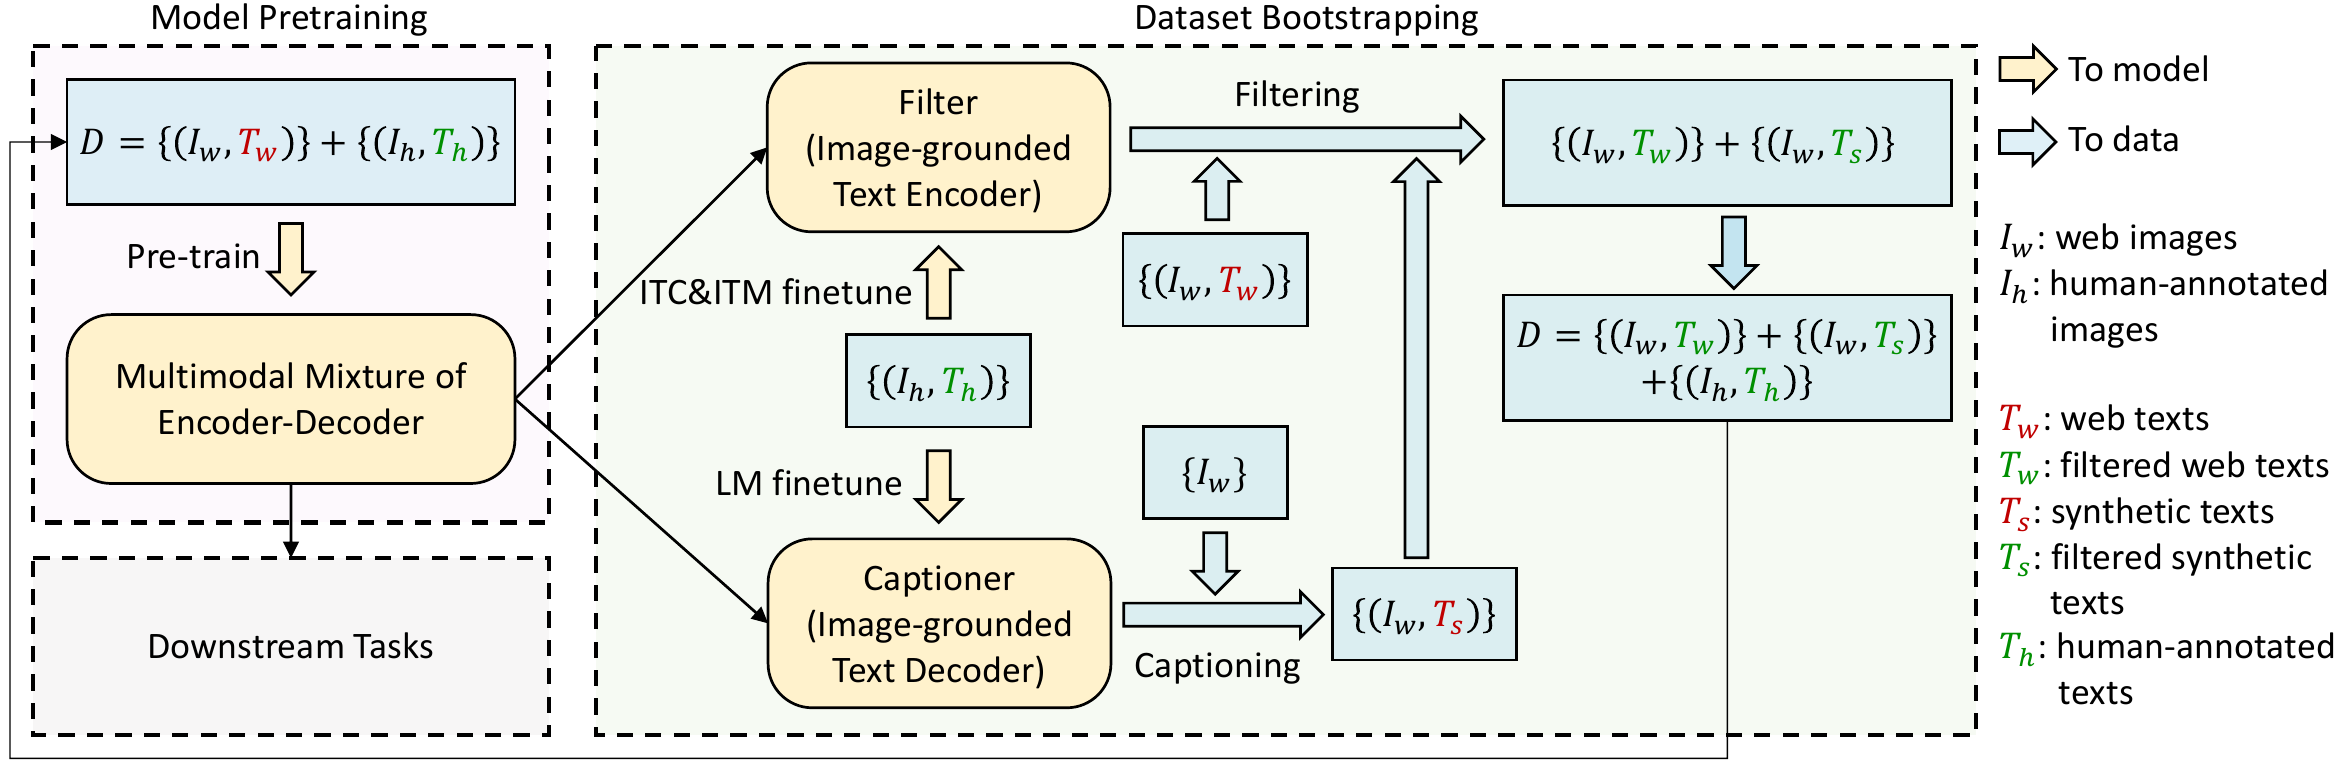
\includegraphics[width=\linewidth,height=0.35\textheight,keepaspectratio]{images/vision-language-models/blip_fig3_capfilt_framework.png}\\[0.1em]
  {\scriptsize $I$: images, $T$: texts; subscripts $w$: web, $s$: synthetic, $h$: human-annotated; red: unfiltered, green: filtered or human. Li et al., \href{https://arxiv.org/abs/2201.12086v2}{arXiv:2201.12086v2}, Figure~3.\par}
  \vspace{0.3em}
  \begin{itemize}\footnotesize\itemsep0.15em
    \item Two copies of the pretrained MED are each fine-tuned, lightly, on COCO captions (covered earlier).
    \item \textbf{Captioner} (grounded decoder, LM): one synthetic caption $T_s$ per web image $I_w$, by \textbf{nucleus sampling}: each token comes from the top tokens whose probabilities sum to $p = 0.9$.
    \item \textbf{Filter} (grounded encoder, ITC and ITM): removes a web text $T_w$ or a synthetic text $T_s$ when its ITM head predicts ``unmatched''.
    \item The kept pairs plus the human pairs pretrain a \textbf{new} model. Data: 14M images (human-annotated COCO and Visual Genome; web caption sets CC3M and CC12M (Conceptual Captions) and SBU Captions) or 129M with 115M LAION images.
  \end{itemize}
\end{frame}

\begin{frame}{What CapFilt Buys}
  \centering
  {\scriptsize
  \begin{tabular}{l c c c c c c c}
    \toprule
    \textbf{Pretraining data} & \textbf{C} & \textbf{F} & \textbf{TR@1} & \textbf{IR@1} & \textbf{B@4} & \textbf{CIDEr} & \textbf{NoCaps CIDEr} \\
    \midrule
    14M images & \xmark & \xmark & 78.4 & 60.7 & 38.0 & 127.8 & 102.2 \\
     & \xmark & \cmark$_B$ & 79.1 & 61.5 & 38.1 & 128.2 & 102.7 \\
     & \cmark$_B$ & \xmark & 79.7 & 62.0 & 38.4 & 128.9 & 103.4 \\
     & \cmark$_B$ beam & \cmark$_B$ & 79.6 & 61.9 & 38.4 & 128.9 & 103.5 \\
     & \cmark$_B$ & \cmark$_B$ & 80.6 & 63.1 & 38.6 & 129.7 & 105.1 \\
    \midrule
    129M images & \xmark & \xmark & 79.6 & 62.0 & 38.8 & 130.1 & 105.4 \\
     & \cmark$_B$ & \cmark$_B$ & 81.9 & 64.3 & 39.4 & 131.4 & 106.3 \\
     & \cmark$_L$ & \cmark$_L$ & 81.2 & 64.1 & 39.7 & 133.3 & 109.6 \\
    \bottomrule
  \end{tabular}\par}
  \vspace{0.3em}
  \raggedright
  {\scriptsize C / F: captioner / filter on ViT-B ($B$) or ViT-L ($L$); beam: beam search, which aims for the most probable caption, instead of nucleus sampling. Pretrained model: ViT-B/16 in every row. TR@1 / IR@1: Recall@1 (share of queries whose top result is correct) for image-to-text / text-to-image retrieval on COCO after fine-tuning; B@4: BLEU-4 (BLEU and CIDEr covered earlier); NoCaps: zero-shot captioning by the COCO-fine-tuned model. Li et al., \href{https://arxiv.org/abs/2201.12086v2}{arXiv:2201.12086v2}, Tables~1, 2 and~4.\par}
  \vspace{0.2em}
  \begin{itemize}\footnotesize\itemsep0.15em
    \item Each module helps alone; together they add 2.2 TR@1 and 2.9 NoCaps CIDEr at 14M. The gain holds at 129M, and ViT-L modules lift NoCaps CIDEr to 109.6.
    \item \textbf{Diversity:} nucleus sampling beats beam search though the filter rejects more of its captions (25\% against 19\%); beam search ``tends to generate safe captions that are common in the dataset'' (Sec.~4.3).
    \item Fine-tune the two modules separately: with shared weights the filter rejects only 8\% of the synthetic captions and every score drops (Table~4).
  \end{itemize}
\end{frame}

\begin{frame}{BLIP-2: Bridging a Frozen Encoder and a Frozen LLM}
  \begin{columns}[T,onlytextwidth]
    \column{0.54\textwidth}
      \begin{itemize}\footnotesize\itemsep0.35em
        \item \textbf{BLIP-2} (Li et al., ICML 2023) freezes a pretrained image encoder and a pretrained LLM and trains only a bridge between them, which cuts compute and keeps what both models already know.
        \item \textbf{Q-Former} (Querying Transformer), initialized from BERT-base: 32 learnable queries of width 768 read the frozen image features by cross-attention. Output $32\times768$, against $257\times1024$ ViT-L/14 features.
        \item \textbf{Frozen encoder:} CLIP ViT-L/14 or EVA-CLIP ViT-g/14 (about 1B parameters). \textbf{Frozen LLM:} OPT (decoder-only, no instruction tuning) or FlanT5 (instruction-tuned encoder-decoder).
        \item \textbf{Two stages:} representation learning with the frozen encoder alone, then generative learning through the frozen LLM.
      \end{itemize}
    \column{0.44\textwidth}
      \centering
      \vspace{0.4em}
      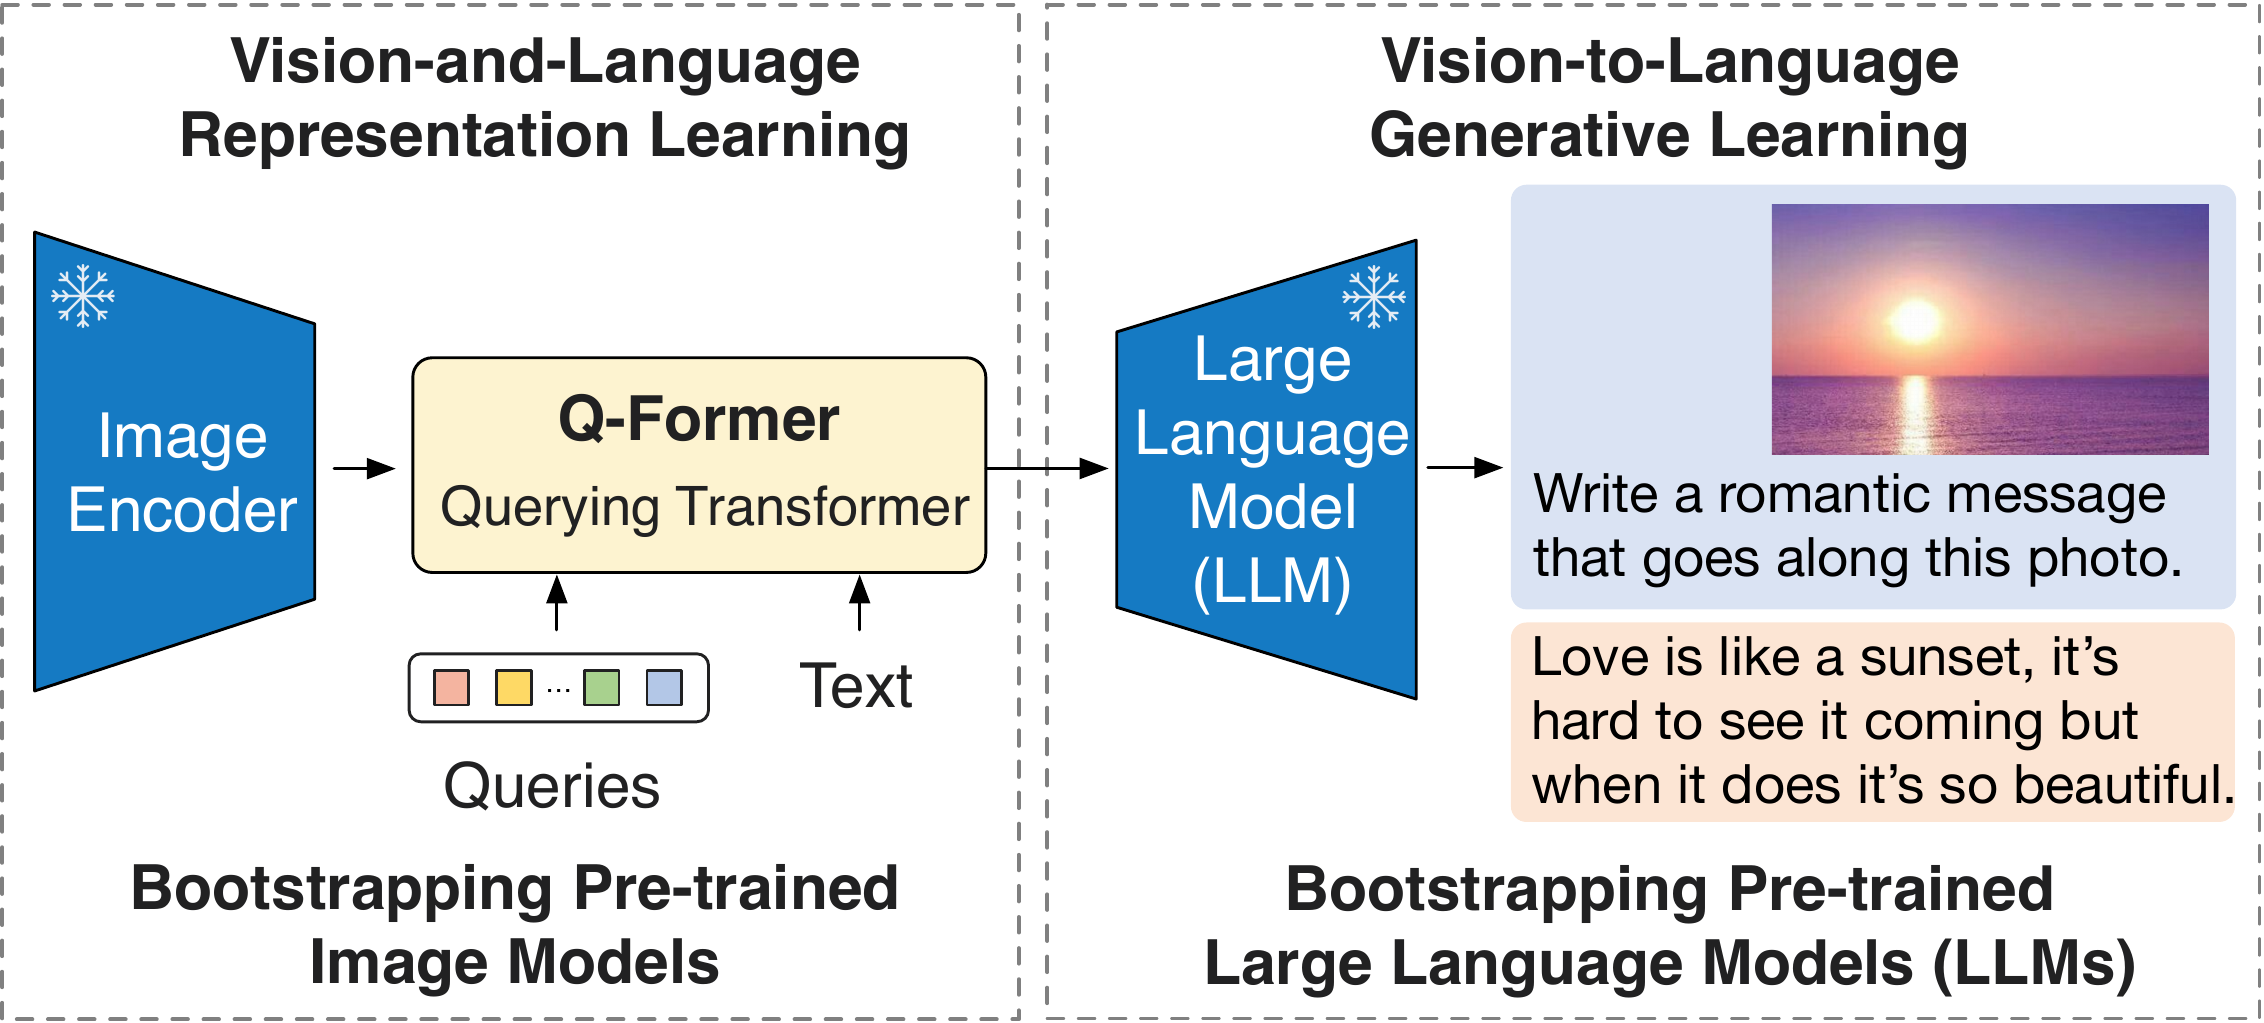
\includegraphics[width=\linewidth,height=0.42\textheight,keepaspectratio]{images/vision-language-models/blip2_fig1_overview.png}\\[0.2em]
      {\scriptsize Snowflake: frozen. Li et al., ``BLIP-2: Bootstrapping Language-Image Pre-training with Frozen Image Encoders and Large Language Models,'' ICML 2023, \href{https://arxiv.org/abs/2301.12597v3}{arXiv:2301.12597v3}, Figure~1.\par}
      \vspace{0.4em}
      \raggedright
      {\scriptsize Largest model (ViT-g with FlanT5-XXL): under 6 days for stage 1 and under 3 days for stage 2 on one machine with 16 A100 (40\,GB) GPUs.\par}
  \end{columns}
  \vspace{0.3em}
  {\footnotesize \textbf{Result:} zero-shot VQAv2 accuracy (test-dev) of 65.0 against 56.3 for Flamingo-80B, which trains 10.2B of its 80B parameters; BLIP-2 trains 188M, 54$\times$ fewer (Table~1; Table~2 lists 108M for this model).\par}
\end{frame}

\begin{frame}{Q-Former: Three Objectives, Three Attention Masks}
  \centering
  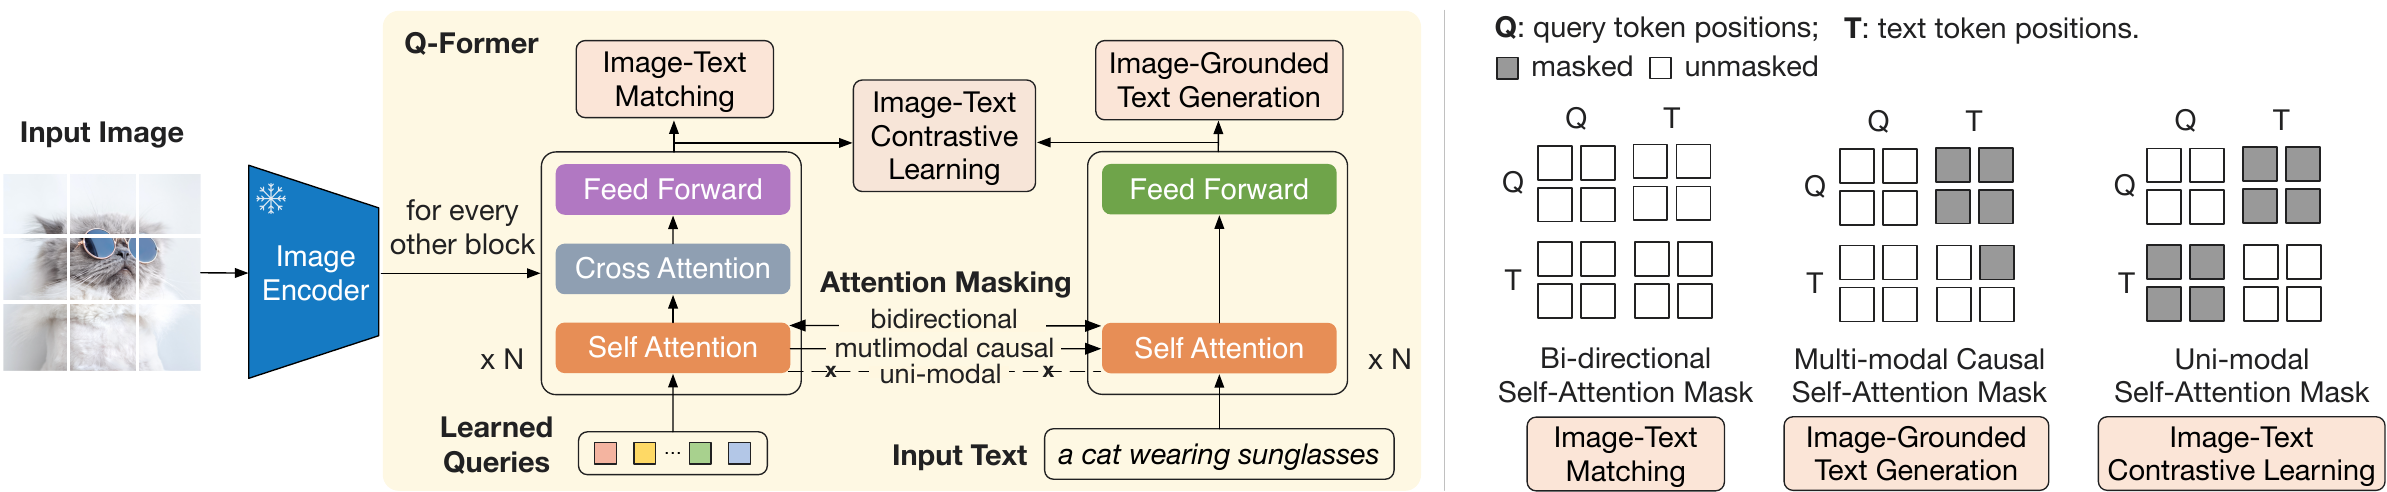
\includegraphics[width=0.92\linewidth,height=0.40\textheight,keepaspectratio]{images/vision-language-models/blip2_fig2_qformer_masks.png}\\[0.1em]
  {\scriptsize Left: queries and text share the self-attention layers; only the queries cross-attend to the frozen encoder, in every other block. Right: one mask per objective (gray: masked). Li et al., \href{https://arxiv.org/abs/2301.12597v3}{arXiv:2301.12597v3}, Figure~2.\par}
  \vspace{0.3em}
  \begin{itemize}\footnotesize\itemsep0.15em
    \item \textbf{ITC, unimodal mask:} queries and text cannot see each other; score $=\max_k s(\mathbf{h}_k,\mathbf{t})$ over query outputs $\mathbf{h}_k$ and the text [CLS] output $\mathbf{t}$; in-batch negatives replace BLIP's queue, as more samples fit per GPU.
    \item \textbf{ITG} (image-grounded text generation)\textbf{, multimodal causal mask:} queries see only queries; text sees all queries and earlier text, so the queries must carry what the caption needs.
    \item \textbf{ITM, bidirectional mask:} all positions see each other; a two-class linear head on each output query, logits averaged; hard negatives as in BLIP.
    \item ITG also helps retrieval (Table~6): adding it to ITC and ITM in COCO fine-tuning lifts Recall@1 from 84.5 to 85.4 (image to text) and from 67.2 to 68.3 (text to image).
  \end{itemize}
\end{frame}

\begin{frame}{BLIP-2 Stage 2: Soft Visual Prompts for the LLM}
  \centering
  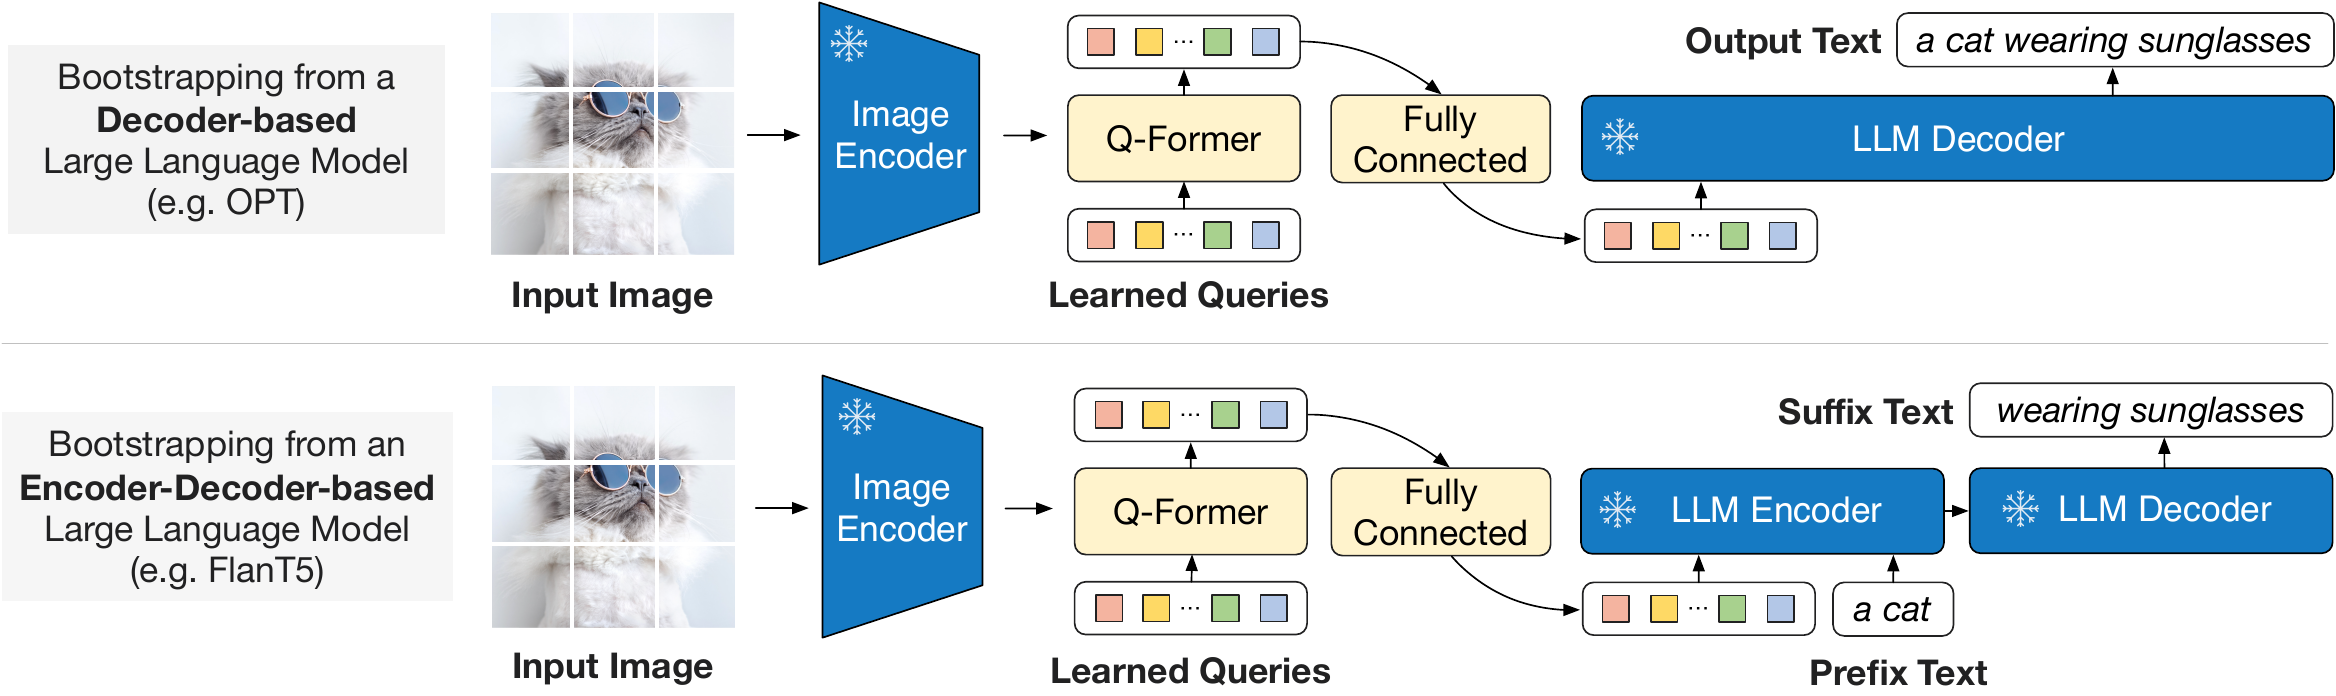
\includegraphics[width=\linewidth,height=0.38\textheight,keepaspectratio]{images/vision-language-models/blip2_fig3_frozen_llm_stage2.png}\\[0.1em]
  {\scriptsize Top: decoder-only LLM (OPT); bottom: encoder-decoder LLM (FlanT5). Li et al., \href{https://arxiv.org/abs/2301.12597v3}{arXiv:2301.12597v3}, Figure~3.\par}
  \vspace{0.3em}
  \begin{itemize}\footnotesize\itemsep0.15em
    \item A linear layer maps the 32 query outputs to the LLM's embedding width; prepended to the text embeddings, they act as \textbf{soft visual prompts}. Only the Q-Former and this layer train.
    \item \textbf{OPT:} language-modeling loss on the text. \textbf{FlanT5:} prefix language modeling; the text is split, the prefix enters the encoder with the visual prompts, the decoder generates the suffix.
    \item Without stage 1, zero-shot VQA is much worse for both LLMs, and with OPT the accuracy drops sharply as training goes on (Figure~5). In-context examples do not help, which the authors trace to one image-text pair per training sample.
    \item \textbf{InstructBLIP} (Dai et al., 2023) also feeds the instruction text to the Q-Former, where it meets the queries in self-attention, so the visual features depend on the task.
  \end{itemize}
\end{frame}
